%\section{Solution design (i mangel af bedre navn}
%This section describes the design of the system as it is implemented. First, system architecture will be presented as to gain an overview of how the system works on a high level. Then the communication between modules will be discussed, following a description of data preprocessing and analysis. At last we discuss how the route planning module of the system works.
\section{System architecture}
\begin{figure}[h!]
  \centering
    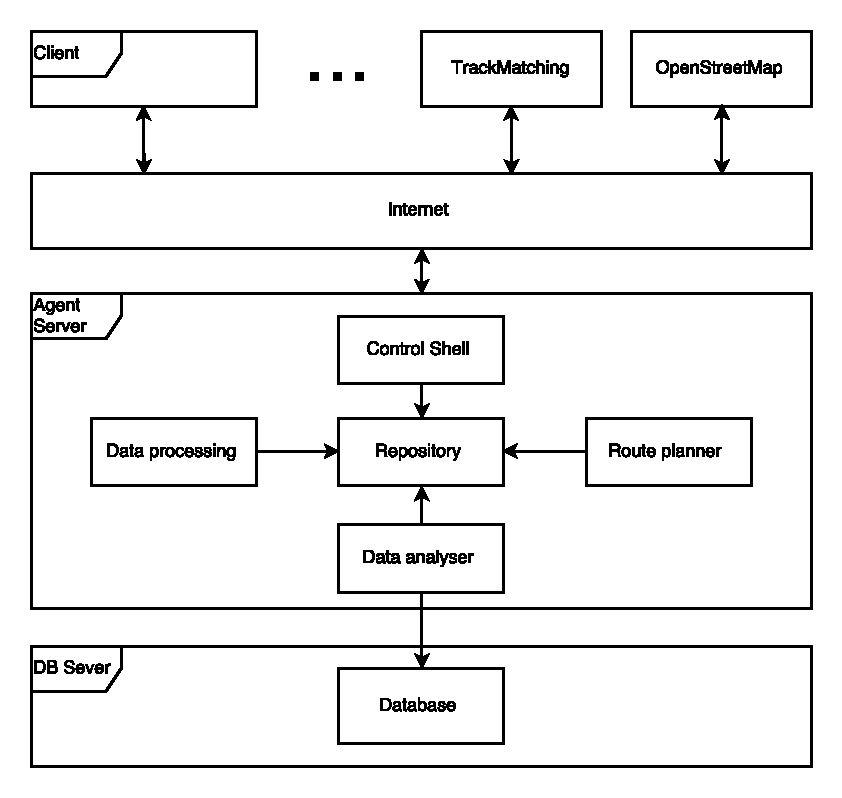
\includegraphics[width=1\textwidth]{figures/architecture.pdf}
    \caption{A course grained system overview.}
    \label{fig:systemoverview}
\end{figure}

The system has been designed as a combination of a client-server and a repository "blackboard" pattern. \figref{fig:systemoverview} shows the overview of the system. The main server module encapsulates most of the processing of the system. The clients represent the GPS-enabled devices that communicates live GPS data through an internet connection to the server, which in turn processes and analyses the data in different subsystems. We use two the external services: TrackMatching to map-match, and OpenStreetMap to obtain map information. They are described in sections \ref{sec:mapmatching} and \ref{sec:mapgeneration}, respectively.

The server architecture is designed as a repository structure, where the solution repository is the shared medium of the subsystems. This architecture is often used when working with artificial intelligence, where the solution is gradually built from different contributing systems, which is why we have chosen this structure of the system.

Initially, the solution repository contains nothing but the problem specification, which is the set of route requests from the clients. The job of the subsystems is to transform the specification into a solution. This is done gradually by invoking the different subsystems to perform operations on the problem specification until a solution can be sent back to the client(s). The control shell module controls which subsystem that should be invoked, based on the contents of the solution repository. 
%The flowchart shows how the user inputs their destination at the start, which sent to a central server together with the source start address. Ther server then uses the data to calculate a route based on the request. The route calculation is based on a initial model of the roadnetwork, such as speedlimits and other restrictions on the roads, and also historical data that have been gathered over time from the users. The route is then sent back to the user, while driving the user will send data back about the drive, this will be the GPS points of the route. This information is then processed and analyzed to check if traffic conditions are as they are supposed to be, and if not the information can be used to recalculate routes for all the drivers which are passing through a that given segment.\todo{review section to describe new architecture}